  \subsection{Análisis de una señal modulada en frecuencia}
    Para la presente experiencia, se emplean los generadores utilizados anteriormente, 
    ya que poseen un \textbf{VCO} (oscilador controlado por tensión), con el 
    cual se pretende generar una señal FM realizando el conexionado de la 
    Figura~\ref{fig:Exp6EsquemaGeneradores}. 

      \begin{figure}[H]
        \centering
          \frame{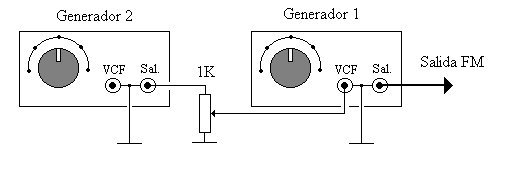
\includegraphics[width=0.8\textwidth]{Imagenes/ActividadPractica/6AnalisisDeUnaSeñalDeFM/EsquemaConexionGeneradores.png}}
          \caption{Conexión de los generadores.}
          \label{fig:Exp6EsquemaGeneradores}
      \end{figure}

    El instrumental utilizado se enseña en la Figura~\ref{fig:Exp6Montaje}.

      \begin{figure}[H]
        \centering
          \frame{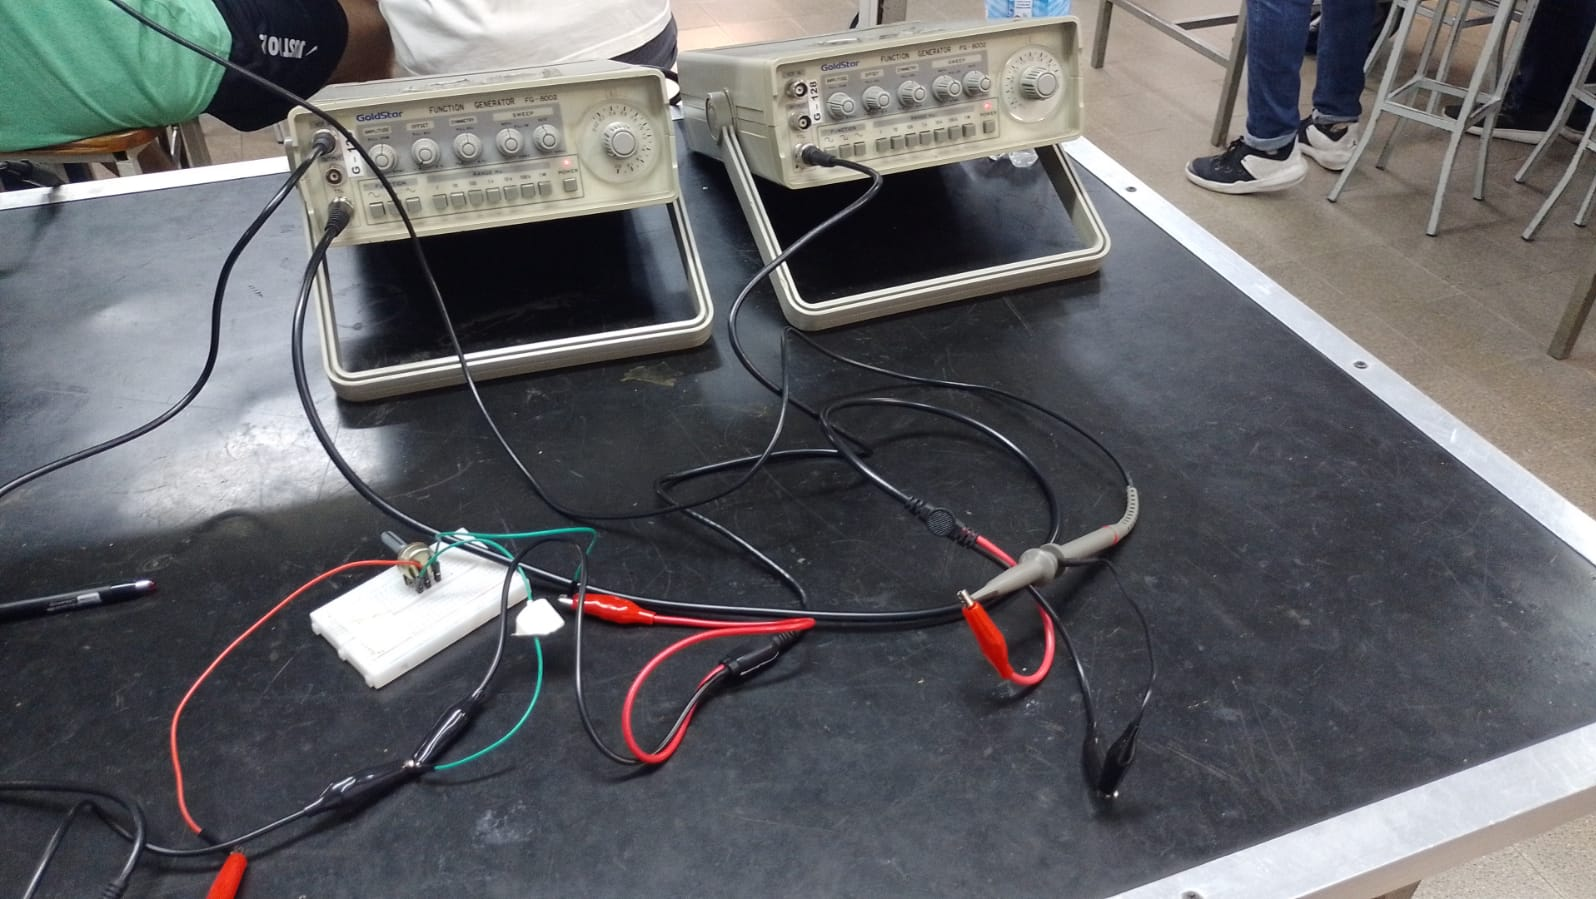
\includegraphics[width=0.48\textwidth]{Imagenes/ActividadPractica/6AnalisisDeUnaSeñalDeFM/Exp6_MontajeCircuito.png}}
          \caption{Montaje del circuito FM.}
          \label{fig:Exp6Montaje}
      \end{figure}    
     
    
    Inicialmente, se procede a ajustar los generadores. La frecuencia de G1 se establece en 
    $\mathbf{f_{G1}=50~kHz}$, y se gira el control de amplitud media vuelta. Por otro lado, se ajusta la 
    frecuencia de G2 a $\mathbf{f_{G2=1~kHz}}$. El seteo de los generadores se observa en la 
    Figura~\ref{fig:Exp6CalibracionGeneradores}.

      \begin{figure}[H]
        \centering
        \begin{subfigure}[H]{0.48\textwidth}
          \frame{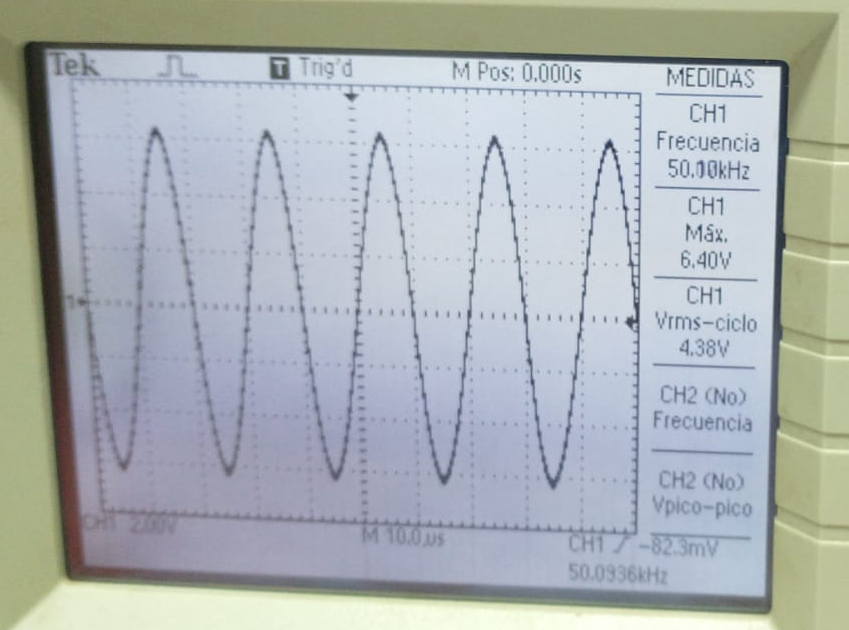
\includegraphics[width=\textwidth]{Imagenes/ActividadPractica/6AnalisisDeUnaSeñalDeFM/Exp6_Calibracion_G1.png}}
          \caption{Calibración del primer generador (G1).}
          \label{fig:Exp6CalibracionG1}
        \end{subfigure}
        \hfill 
        \begin{subfigure}[H]{0.48\textwidth}
          \frame{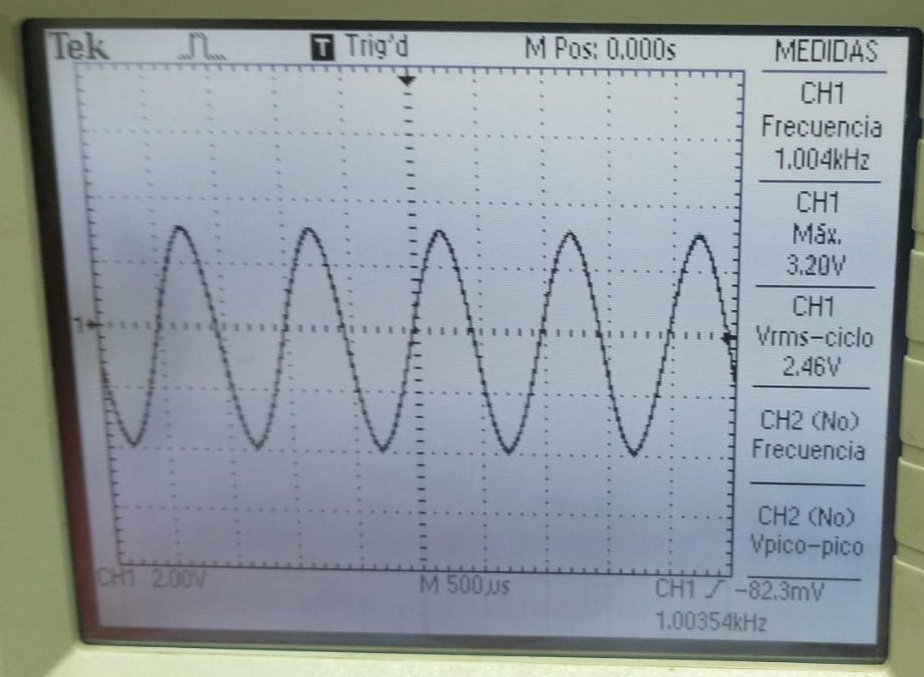
\includegraphics[width=\textwidth]{Imagenes/ActividadPractica/6AnalisisDeUnaSeñalDeFM/Exp6_Calibración_G2.jpg}}
          \caption{Calibración del segundo generador (G2).}
          \label{fig:Exp6CalibracionG2}
        \end{subfigure}

        \caption{Calibración de los generadores.}
        \label{fig:Exp6CalibracionGeneradores}
      \end{figure}

    Luego se procede a configurar el osciloscopio. Se coloca la base de tiempos  
    en $\mathbf{1~ms/div}$, con el control SEC/DIV, como muestra la Figura~\ref{fig:Exp6SeñalFM1ms}.

      \begin{figure}[H]
        \centering
          \frame{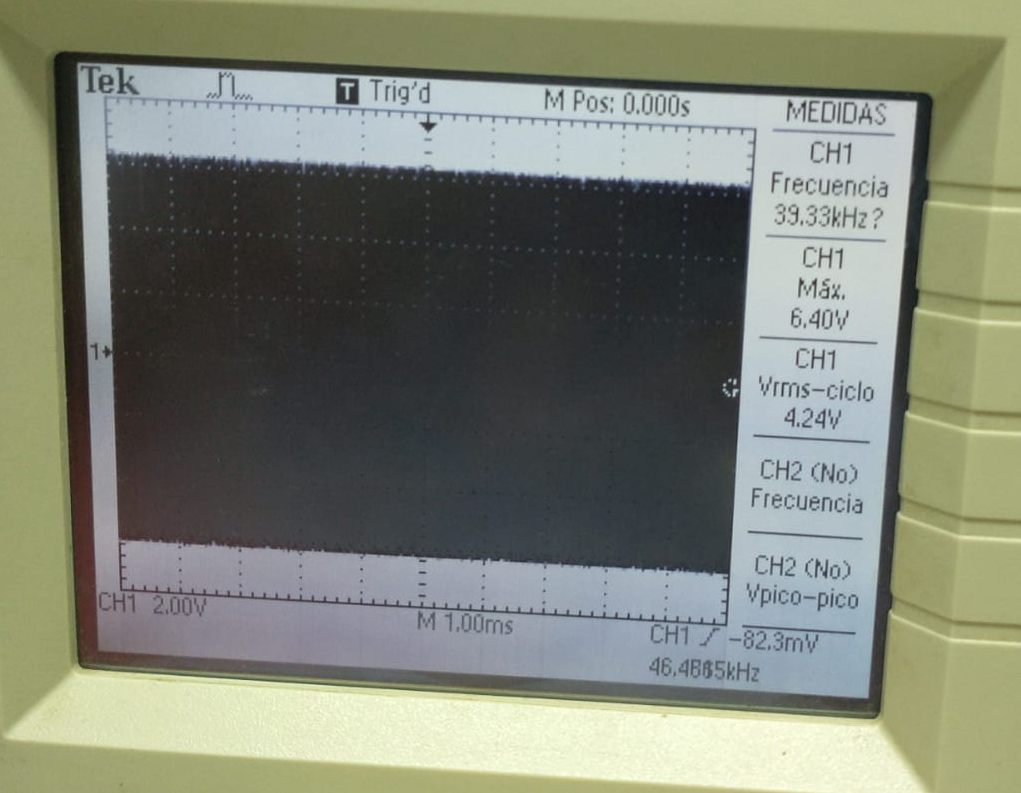
\includegraphics[width=0.5\textwidth]{Imagenes/ActividadPractica/6AnalisisDeUnaSeñalDeFM/Exp6_SeñalDeSalidaCon1msPorDiv.png}}
          \caption{Señal modulada en frecuencia con base de tiempos de $1~ms$.}
          \label{fig:Exp6SeñalFM1ms}
      \end{figure}

    Siguiendo el procedimiento, se configura el menú matemáttico de la siguiente manera:
    \textbf{Hanning}, \textbf{Zoom X10}, y modo adquisición \textbf{Promedio} en 
    64 muestras. La salida FM configurada, se observa en frecuencia en la Figura~\ref{fig:Exp6SeñalFMConfigurada}.

      \begin{figure}[H]
        \centering
        \begin{subfigure}[H]{0.48\textwidth}
          \frame{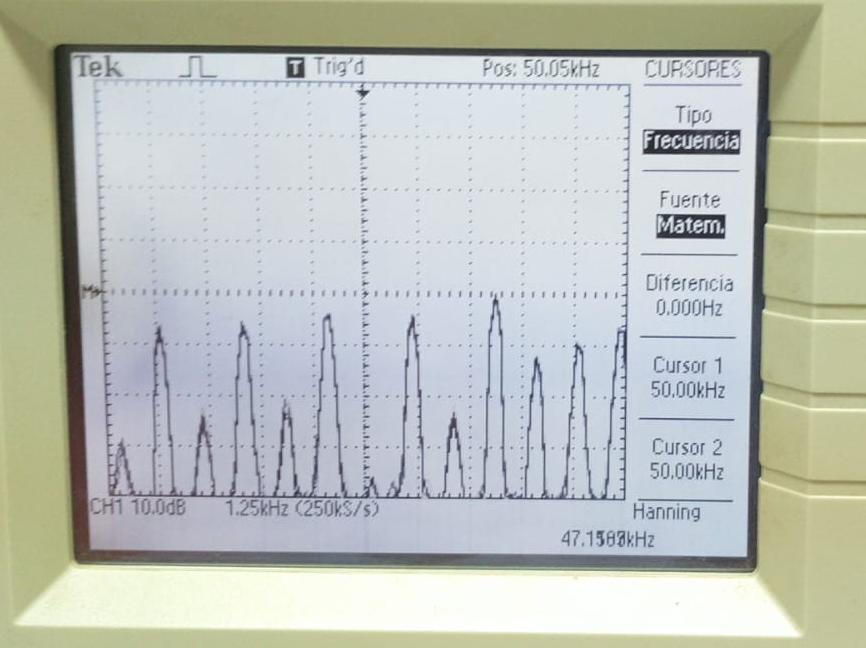
\includegraphics[width=\textwidth]{Imagenes/ActividadPractica/6AnalisisDeUnaSeñalDeFM/Exp6_SalidaFMEnFrecuenciaConfigurada.png}}
          \caption{FM con promedios.}
          \label{fig:Exp6SeñalFM}
        \end{subfigure}
        \hfill 
        \begin{subfigure}[H]{0.48\textwidth}
          \frame{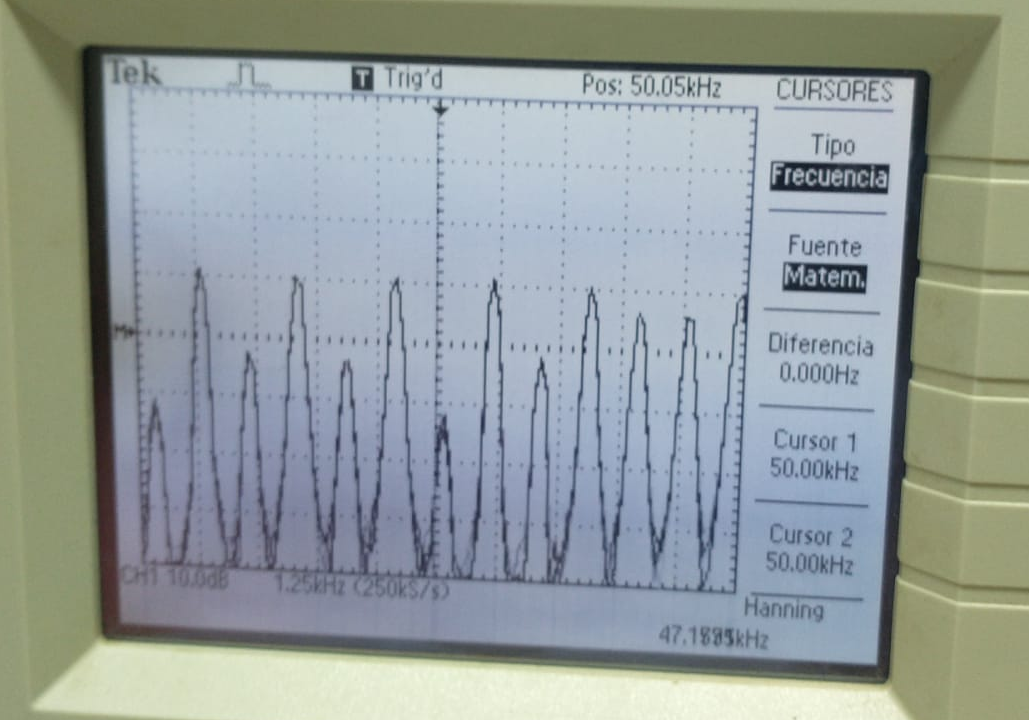
\includegraphics[width=\textwidth]{Imagenes/ActividadPractica/6AnalisisDeUnaSeñalDeFM/Exp6_SalidaFMEnFrecuenciaAdqNormal.png}}
          \caption{Adquisición normal.}
          \label{fig:Exp6SeñalFMAdquisicionNormal}
        \end{subfigure}
        \caption{Generación de señal FM observada en frecuencia.}
        \label{fig:Exp6SeñalFMConfigurada}
      \end{figure}

    Se procede a modificar el índice de modulación, el cual responde a la 
    siguiente ecuación:

    \begin{equation*}
      m_{f}=\dfrac{\Delta_{f}}{f_{m}}~,
    \end{equation*}
    con lo cual, se debe variar la frecuencia de la onda modulante buscando obtener 
    un índice de modulación de \textbf{2.4}, el cual corresponde a una modulación sin 
    portadora. El resultado se observa en la 
    Figura~\ref{fig:Exp6SeñalFMindice2_4}.

      \begin{figure}[H]
        \centering
        \begin{subfigure}[H]{0.48\textwidth}
          \frame{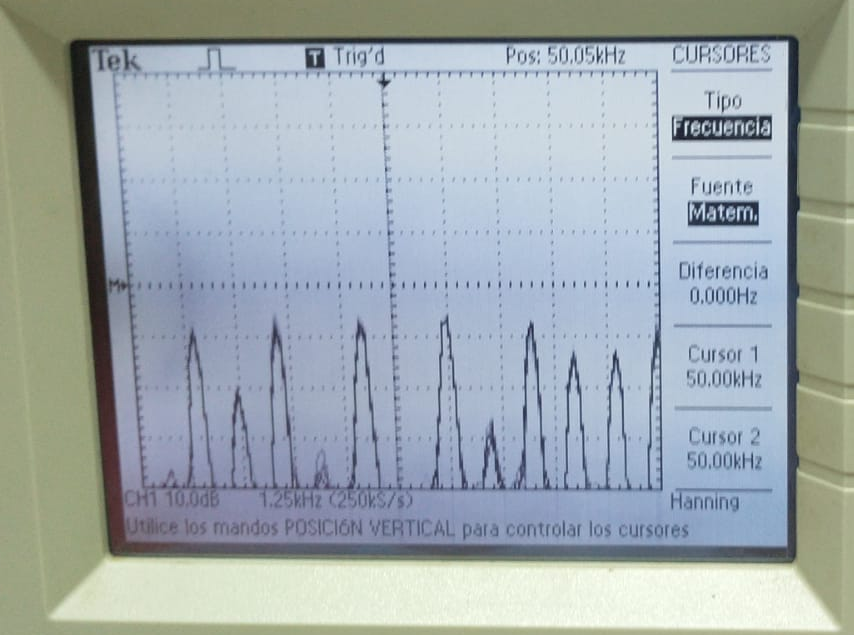
\includegraphics[width=\textwidth]{Imagenes/ActividadPractica/6AnalisisDeUnaSeñalDeFM/Exp6_SalidaFMconindice2_4yPromedios.png}}
          \caption{Salida FM usando adquisición promedio.}
          \label{fig:Exp6SeñalFMIndice2_4AdquisicionPromedio}
        \end{subfigure}
        \hfill 
        \begin{subfigure}[H]{0.48\textwidth}
          \frame{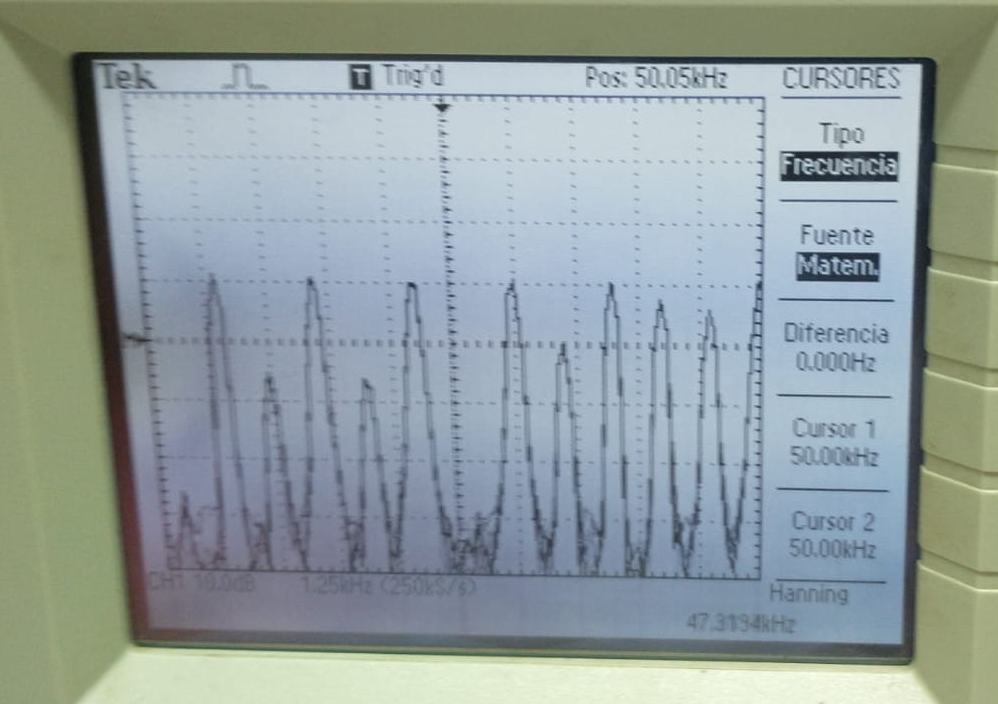
\includegraphics[width=\textwidth]{Imagenes/ActividadPractica/6AnalisisDeUnaSeñalDeFM/Exp6_SalidaFMindice2_4SinPromedios2.png}}
          \caption{Salida FM usando adquisición normal.}
          \label{fig:Exp6SeñalFMIndice2_4AdquisicionNormal}
        \end{subfigure}
        \caption{Generación de señal FM observada en frecuencia.}
        \label{fig:Exp6SeñalFMindice2_4}
      \end{figure}   

    A continuación, se disminuye ligeramente el índice de modulación y se 
    observa el cambio en el espectro. Dicho cambio, se visualiza en la 
    Figura~\ref{fig:Exp6SeñalFMIndiceDisminuido}.

      \begin{figure}[H]
        \centering
          \frame{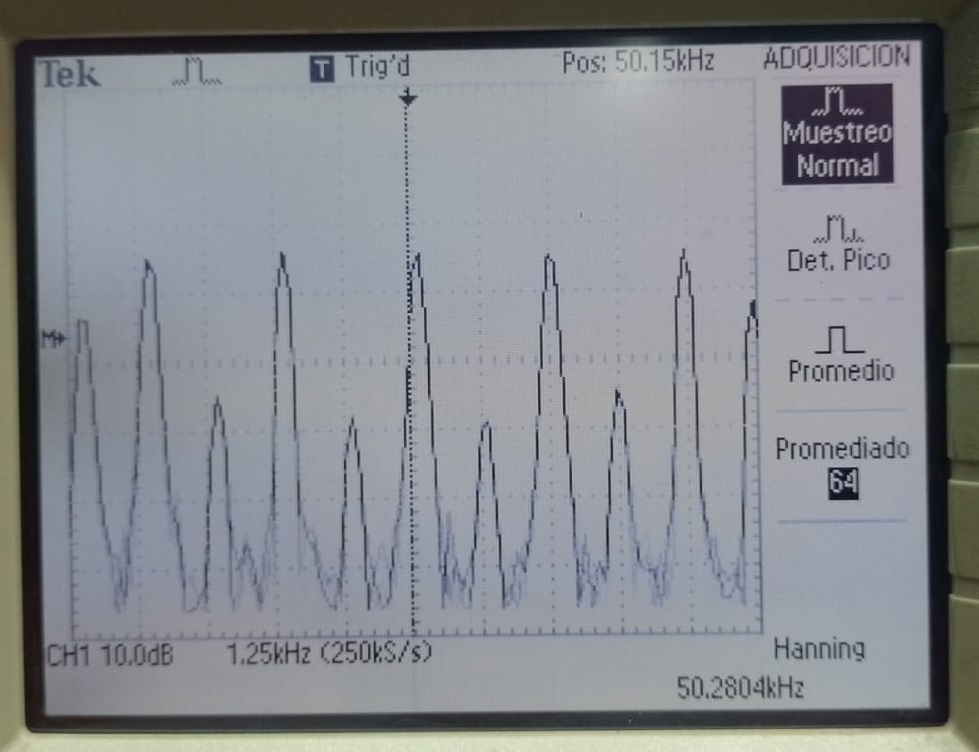
\includegraphics[width=0.5\textwidth]{Imagenes/ActividadPractica/6AnalisisDeUnaSeñalDeFM/Exp6_SalidaFMindiceligeramentedisminuido.png}}
          \caption{Índice ligeramente disminuido.}
          \label{fig:Exp6SeñalFMIndiceDisminuido}
      \end{figure}
    
    Se procede a cambiar la salida de onda modulante (generador G2), a onda 
    cuadrada y triangular. Se observa el cambio en el espectro en la 
    Figuras~\ref{fig:Exp6SeñalFMModulanteCuadrada} y 
    \ref{fig:Exp6SeñalFMModulanteTriangular} para señal 
    cuadrada y triangular respectivamente, además se cambia el tipo 
    de ventana entre Hanning, Rectangular y Flattop.

      \begin{figure}[H]
        \centering
        \begin{subfigure}[H]{0.40\textwidth}
          \frame{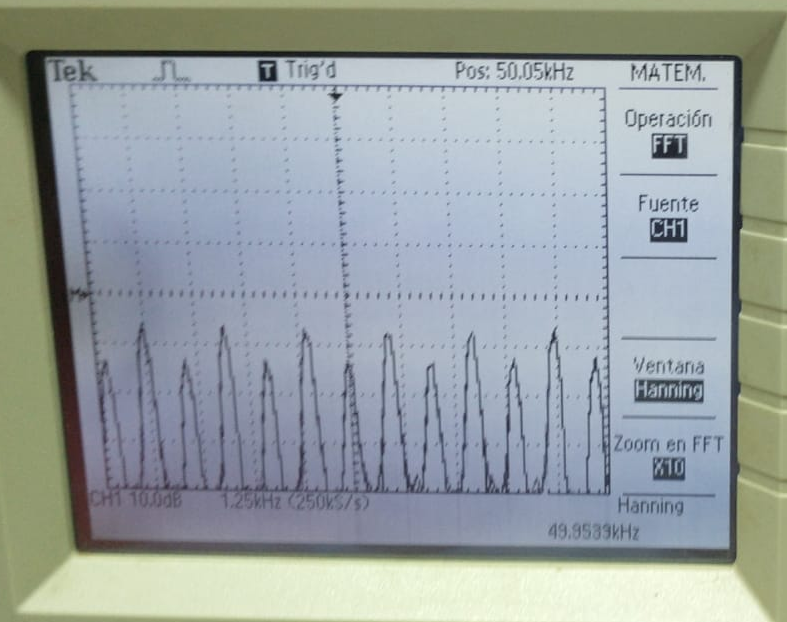
\includegraphics[width=\textwidth]{Imagenes/ActividadPractica/6AnalisisDeUnaSeñalDeFM/Exp6_SeñalFMConmodulanteCuadradaSinPromedios.png}}
          \caption{Con ventana Hanning.}
          \label{fig:Exp6SeñalFMModulanteCuadradaHanning}
        \end{subfigure}
        \hfill 
        \begin{subfigure}[H]{0.40\textwidth}
          \frame{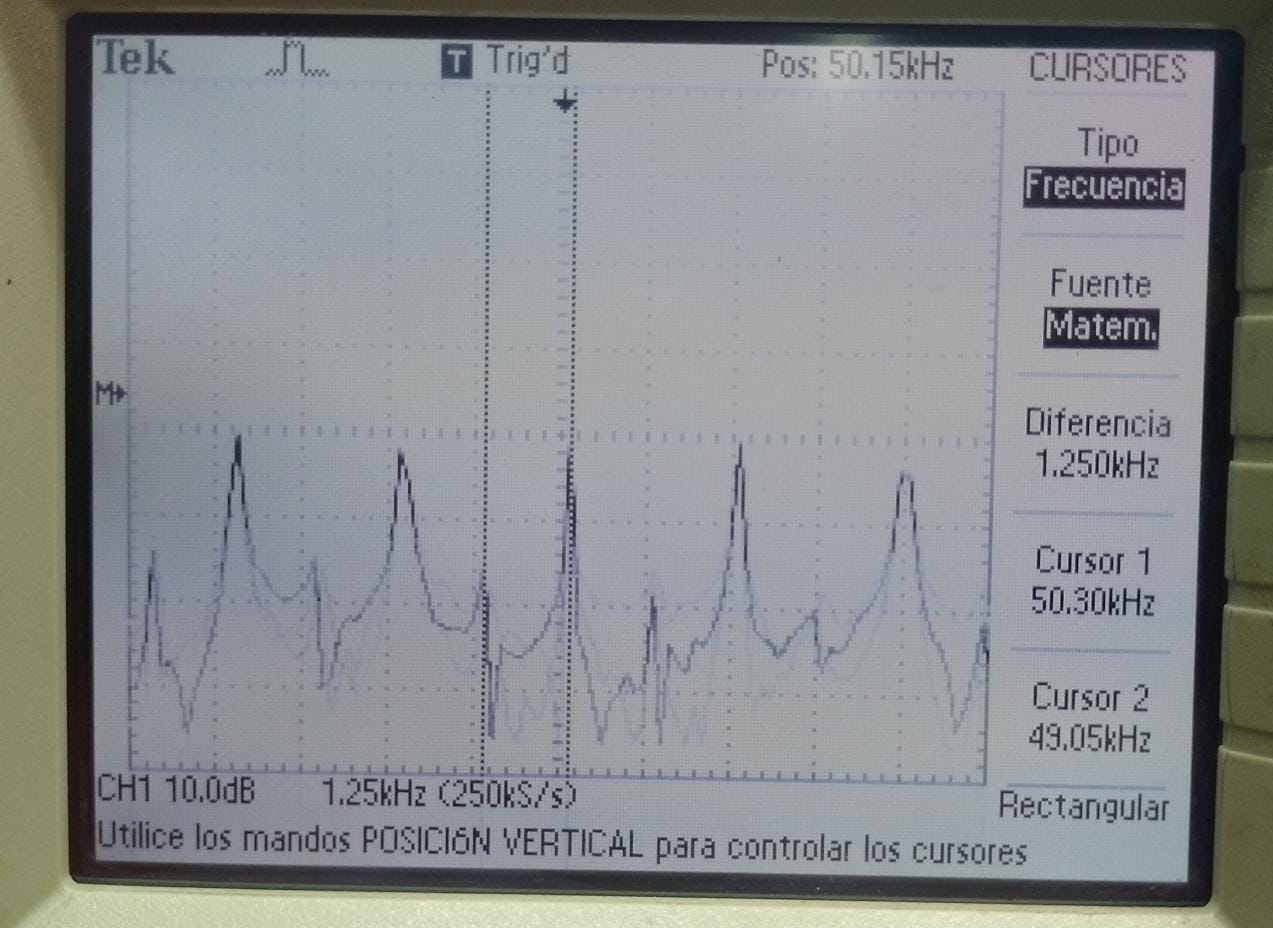
\includegraphics[width=\textwidth]{Imagenes/ActividadPractica/6AnalisisDeUnaSeñalDeFM/Exp6_SeñalFMConModulanteCuadradaSinPromediosVentanaRectangular.png}}
          \caption{Con ventana Rectangular.}
          \label{fig:Exp6SeñalFMModulanteCuadradaRectangular}
        \end{subfigure}
        \begin{subfigure}[H]{0.40\textwidth}
          \frame{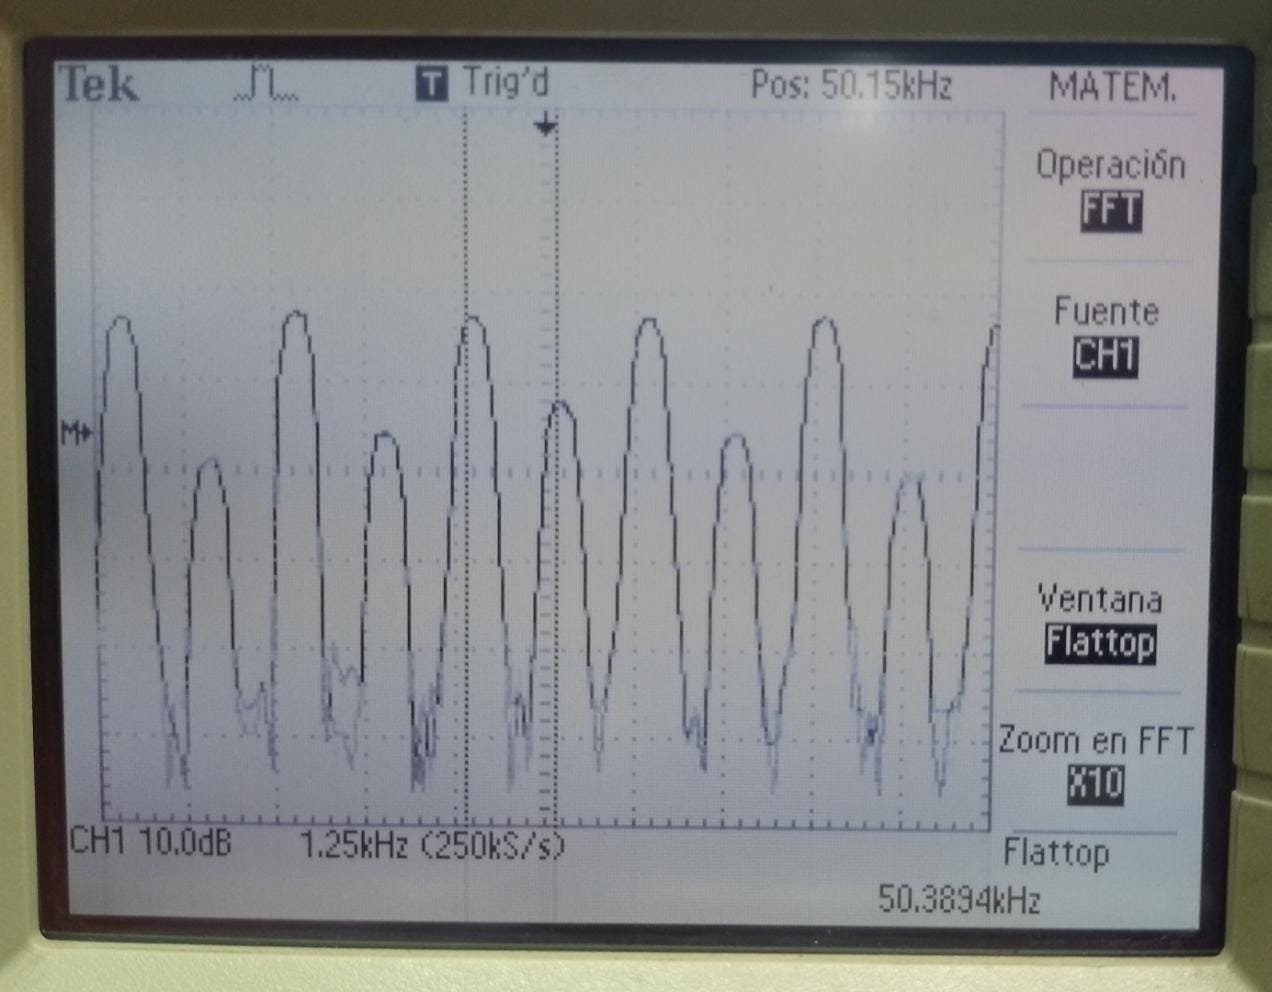
\includegraphics[width=\textwidth]{Imagenes/ActividadPractica/6AnalisisDeUnaSeñalDeFM/Exp6_SeñalFMConModulanteTriángularVentanaFlattop.png}}
          \caption{Con ventana Flattop.}
          \label{fig:Exp6SeñalFMModulanteCuadradaFlattop}
        \end{subfigure}
        \caption{Onda cuadrada como señal modulante.}
        \label{fig:Exp6SeñalFMModulanteCuadrada}
      \end{figure}   

      Se inyecta una señal triangular y se ven distintas ventanas.

      \begin{figure}[H]
        \centering
        \begin{subfigure}[H]{0.48\textwidth}
          \frame{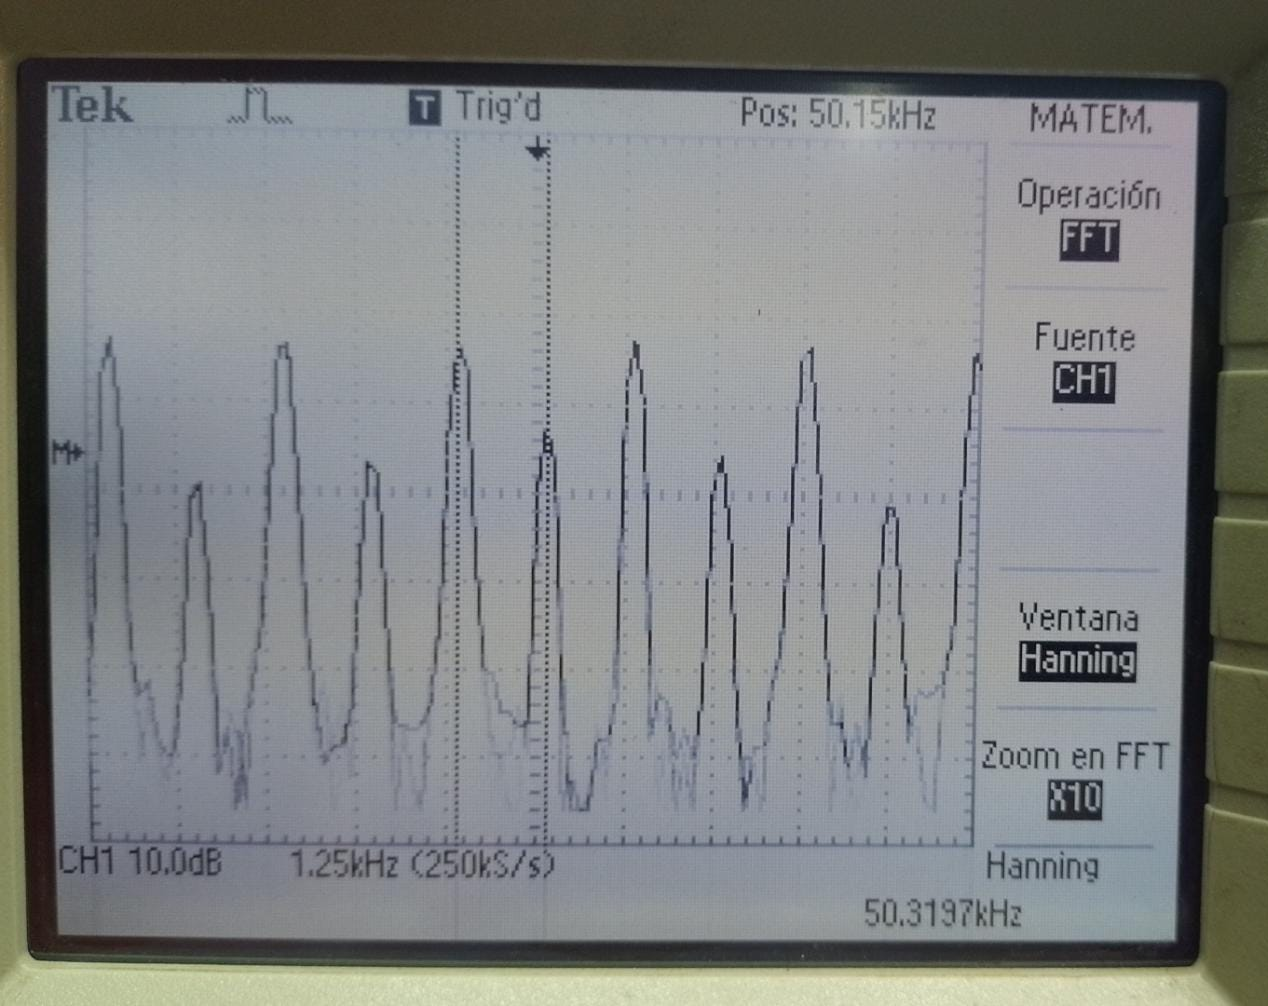
\includegraphics[width=\textwidth]{Imagenes/ActividadPractica/6AnalisisDeUnaSeñalDeFM/Exp6_SeñalFMConmodulanteTriángularSinPromedioVentanaHanning.png}}
          \caption{Con ventana Hanning.}
          \label{fig:Exp6SeñalFMModulanteTriangularHanning}
        \end{subfigure}
        \hfill 
        \begin{subfigure}[H]{0.48\textwidth}
          \frame{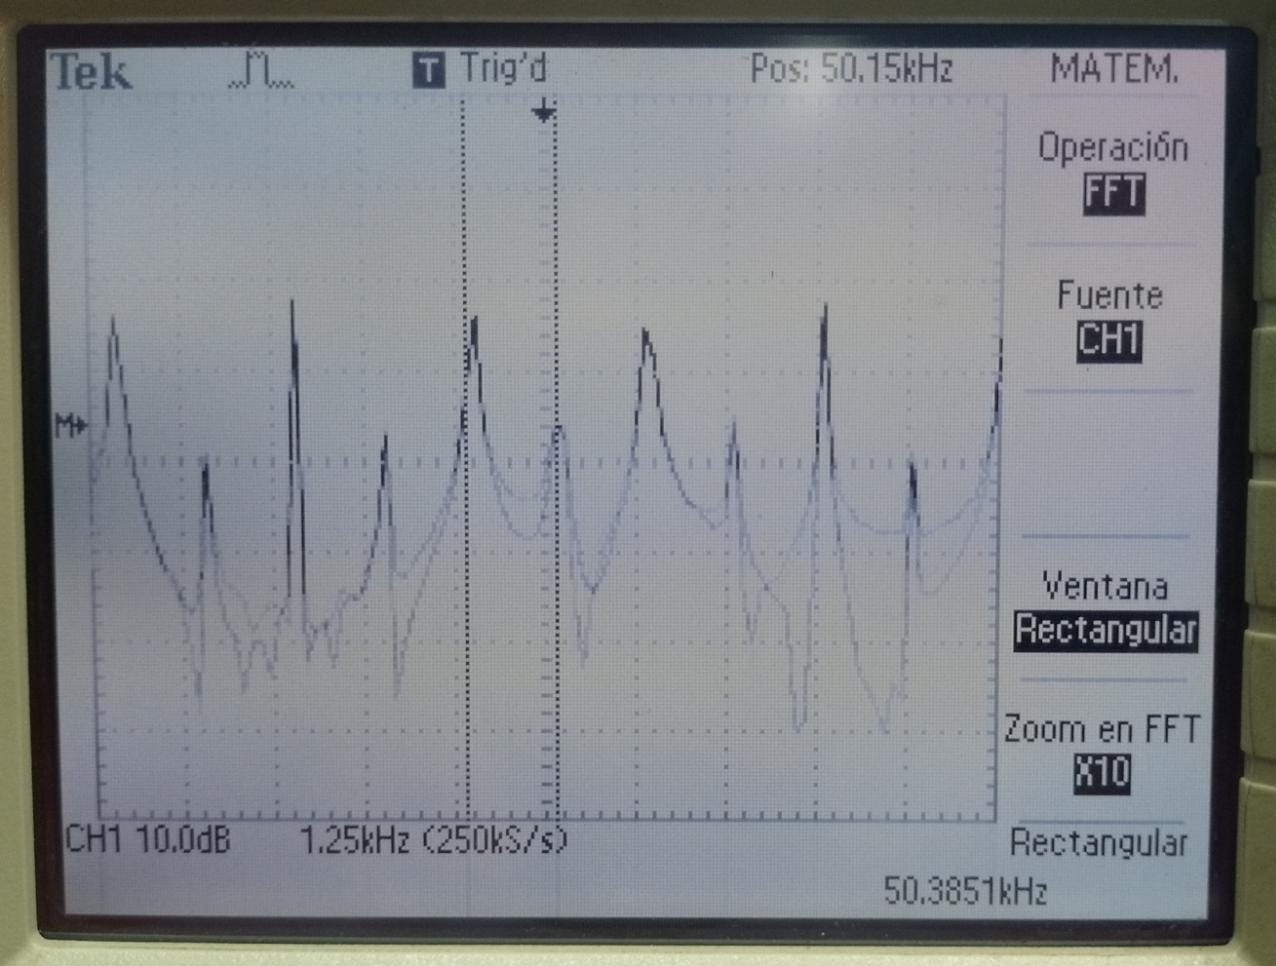
\includegraphics[width=\textwidth]{Imagenes/ActividadPractica/6AnalisisDeUnaSeñalDeFM/Exp6_SeñalFMConmodulanteTriángularSinPromedioVentanaRectangular.png}}
          \caption{Con ventana Rectangular.}
          \label{fig:Exp6SeñalFMModulanteTriangularRectangular}
        \end{subfigure}
       \begin{subfigure}[H]{0.48\textwidth}
          \frame{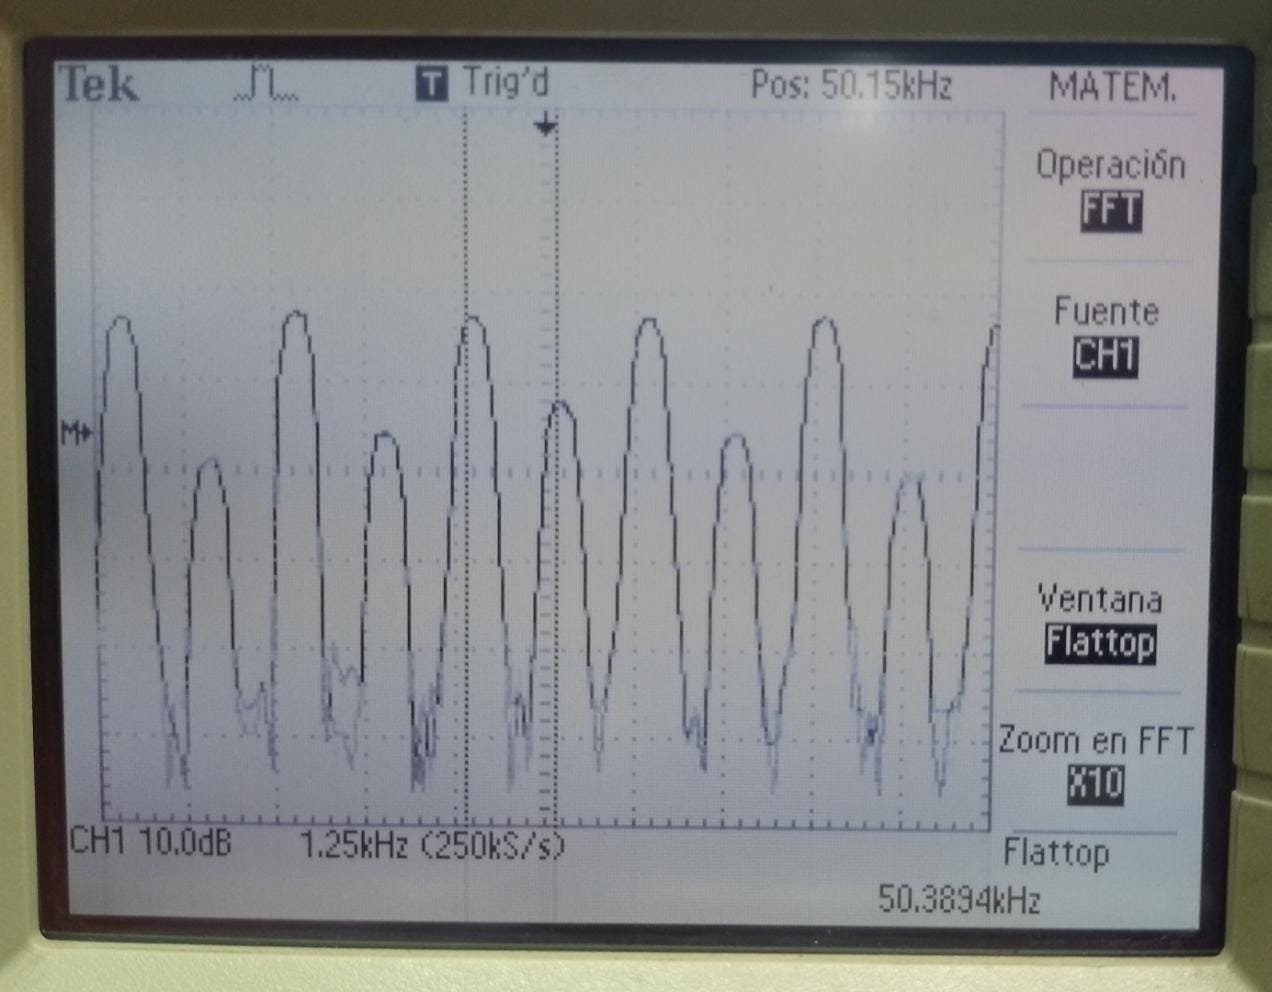
\includegraphics[width=\textwidth]{Imagenes/ActividadPractica/6AnalisisDeUnaSeñalDeFM/Exp6_SeñalFMConModulanteTriángularVentanaFlattop.png}}
          \caption{Con ventana Flattop.}
          \label{fig:Exp6SeñalFMModulanteTriangularFlattop}
        \end{subfigure}
        \caption{Onda triangular como señal modulante.}
        \label{fig:Exp6SeñalFMModulanteTriangular}
      \end{figure}         

    Se procede a efectuar la medición de frecuencias de portadora y de bandas 
    laterales, para determinar el valor de la frecuencia modulante. Se emplea como 
    señal modulante una onda senoidal, y se setea ventana \textbf{Hanning} para realizar 
    la medición.

      \begin{equation}
        f_{Modulante}=|f_{Portadora}-f_{BLateral}|
        \label{eqn:Exp6CalculoModulante}
      \end{equation}

      \begin{figure}[H]
        \centering
        \begin{subfigure}[H]{0.48\textwidth}
          \frame{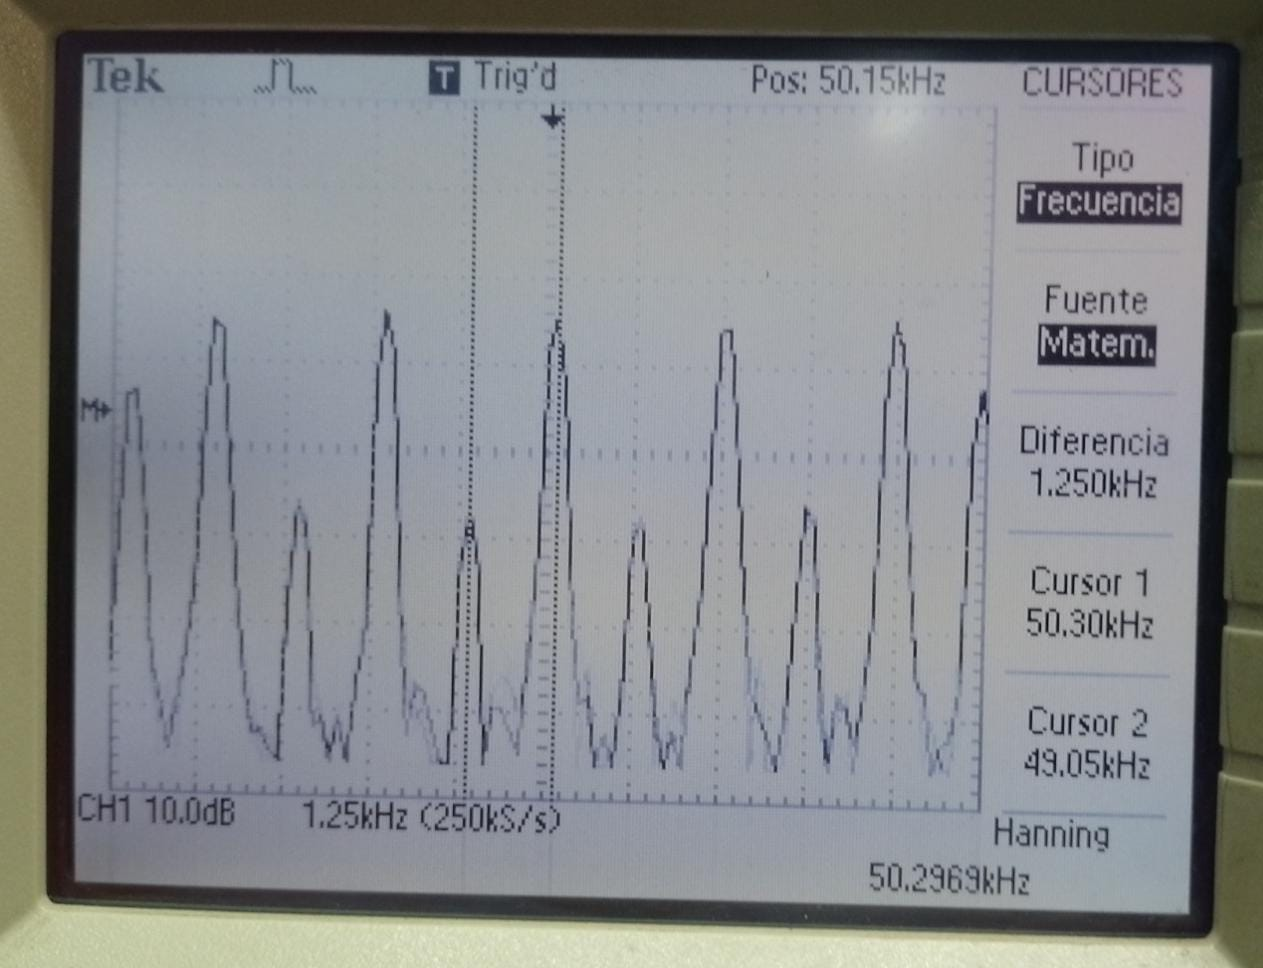
\includegraphics[width=\textwidth]{Imagenes/ActividadPractica/6AnalisisDeUnaSeñalDeFM/Exp6_SeñalFMMedicionDeFrecModulante_DiferenciaEntrePortadoraYBandaI.png}}
          \caption{Diferencia con banda lateral inferior.}
          \label{fig:Exp6SeñalFMDifBandaLateralIzq}
        \end{subfigure}
        \hfill 
        \begin{subfigure}[H]{0.48\textwidth}
          \frame{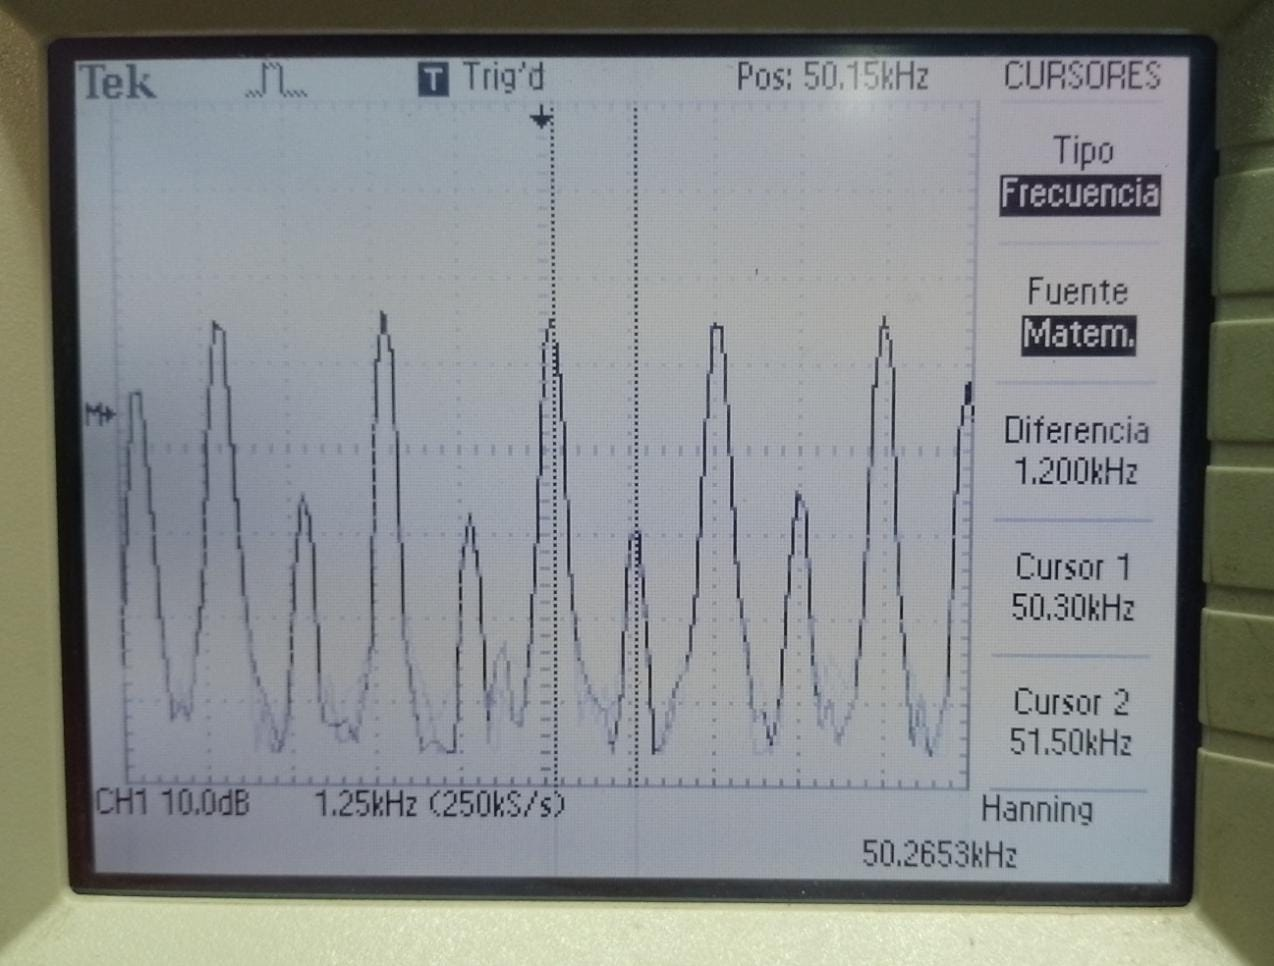
\includegraphics[width=\textwidth]{Imagenes/ActividadPractica/6AnalisisDeUnaSeñalDeFM/Exp6_SeñalFMMedicionDeFrecModulante_DiferenciaEntrePortadoraYBandaS.png}}
          \caption{Diferencia con banda lateral superior.}
          \label{fig:Exp6SeñalFMDifBandaLateralDer}
        \end{subfigure}
      \end{figure}  

      De la Figura~\ref{fig:Exp6SeñalFMDifBandaLateralDer} se observa un valor de 
      $f_{Portadora}=50,3~kHz$ y $f_{BLateral}=51,5~kHz$, reemplazando éstos valores en 
      la ecuación~(\ref{eqn:Exp6CalculoModulante}) se tiene 

      \begin{align*}
        f_{Modulante}=|50,3~kHz-51,5~kHz| \hspace{20pt} \therefore \hspace{20pt} \boxed{f_{Modulante}=1,2~[kHz]}~.
      \end{align*}
    
